\section{Figuras musicais, pausas e durações}
\index{Música!Figuras musicais}
\index{Música!Figuras rítmicas}
\label{sec:figurasmusicais}
As figuras musicais também chamada figuras rítmicas \cite[pp. 16]{alves2004teoria}, 
são um conjunto de sinais (desenhos), criadas pra indicar a relação 
entre as \hyperref[sec:pos:Duracion]{\textbf{durações}} dos sons \cite[pp. 20]{medteoria}.
Assim, podemos ver na coluna dois da Tabela \ref{tab:abc-noteslengthbasic}
 um conjunto de 6 destas figuras musicais; 
a primeira coluna representa a longitude temporal (\hyperref[sec:pos:Duracion]{\textbf{duração}}) de cada uma destas figuras;
porem, todos estas durações são relativas ao valor temporal $S$, em segundos, de uma figura \Ganz.
A terceira coluna da tabela contem os nomes de cada uma destas figuras musicais. 
\begin{table}[h]
\centering
\begin{tabular}{|c||c|c||c|c|}
\hline
Duração & Figura & Nome de figura & Pausa & Nome de pausa\\ \hline
\hline
$S$    & \Ganz   & Semibreve    & \GaPa  & Pausa de Semibreve \\ \hline
$S/2$  & \Halb   & Mínima       & \HaPa  & Pausa de Mínima \\ \hline
$S/4$  & \Vier   & Semínima     & \ViPa  & Pausa de Semínima \\ \hline
$S/8$  & \Acht   & Colcheia     & \AcPa  & Pausa de Colcheia \\ \hline
$S/16$ & \Sech   & Semicolcheia & \SePa  & Pausa de Semicolcheia \\ \hline
$S/32$ & \Zwdr   & Fusa         & \ZwPa  & Pausa de fusa  \\ \hline  
\end{tabular}
\caption{Duração e símbolos de algumas figuras musicais}
\label{tab:abc-noteslengthbasic}
\end{table}


\begin{example}
Se decidimos criar uma sequencia rítmica assoviando um único tom, porem
distribuindo os tempos de duração como: Longo, curto, curto; 
repetindo esta sequencia quatro vesses. 
Poderíamos escrever esta sequencia usando figuras musicais numa representação como a mostrada na Figura \ref{fig:abc-figurasexample1}.
É importante ressaltar que assumimos que  um sonido longo dura no tempo exatamente o dobro que um curto, 
e que decidimos\footnote{É escolhida uma semínima porem pode ter sido escolhida 
qualquer outra figura, dado que o valor $S$ não está definido.}
representar um sonido de longa duração como uma semínima.

Para entender melhor a representação com figuras musicais, 
podemos ir a uma representação alternativa com um gráfico da potencia sonora na execução dos sons,
como é representado na Figura \ref{fig:forma-figurasexample1b}.
É fácil perceber como a potencia do som se mantêm, ate justo antes de iniciar 
o seguinte som, de modo que não existem silêncios na sequencia rítmica.
\end{example} 




\begin{figure}[h]
    \centering
    \begin{subfigure}[b]{0.9\textwidth}
 \begin{abc}[name=abc-figurasexample1]
% abcm2ps figurasexample1.abc  -O figurasexample1.ps
% ps2epsi figurasexample1.ps figurasexample1.eps
%
X: 1 % start of header
K: none stafflines=0 %K: C %% Escala de C mayor %
M:  none % M: 2/4
%T: Contratempo num compasso binário
V:1 clef=none stem=up %name="Ritmo 1"   sname="Ritmo 1"
%
[V:1] | B2 B1 B1 B2 B1 B1 B2 B1 B1 B2  B1 B1   |
%       
\end{abc}
	\caption{Sequencia rítmica usando semínimas e colcheias.}
	\label{fig:abc-figurasexample1}
    \end{subfigure}
    ~%add desired spacing between images, e. g. ~, \quad, \qquad, \hfill etc. 
      %(or a blank line to force the subfigure onto a new line)
    \begin{subfigure}[b]{0.9\textwidth}
        
\includegraphics[width=\textwidth]{chapters/cap-musica-basica/forma-figurasexample1.eps}
        \caption{Sequencia rítmica usando um gráfico indicando a potencia do sonido.}
        \label{fig:forma-figurasexample1b}
    \end{subfigure}
    \caption{Sequencia rítmica.}\label{fig:total-figurasexample1}
\end{figure}


Por outro lado, assim como a duração do tempo de execução de cada som precisa uma grafia,
os silêncios ou pausas, também precisam ser indicados. 
De modo que, para cada figura musical existe uma grafia que indica um silencio da mesma duração temporal,
como pode ser visto na quarta coluna da Tabela \ref{tab:abc-noteslengthbasic}.
O nome de cada uma destas pausas está descrito na quinta coluna da mesma tabela.

\begin{example}
Similarmente ao exemplo anterior, se decidimos criar uma sequencia rítmica assoviando um único tom, porem
intercalando sons e silêncios, criaremos um padrão rítmico como na Figura \ref{fig:total-figurasexample2}.

Podemos entender melhor a representação com figuras musicais, 
usando a representação com um gráfico da potencia sonora na execução dos sons,
como é representado na Figura \ref{fig:forma-figurasexample2}.
Nela percebemos como a potencia do som se mantêm durante a longitude de tempo estipulada pela figura musical, 
ate justo antes de iniciar o silencio, indicado por uma linha reta horizontal.
\end{example} 

\begin{figure}[h]
    \centering
    \begin{subfigure}[b]{0.9\textwidth}
 \begin{abc}[name=abc-figurasexample2]
% abcm2ps figurasexample2.abc  -O figurasexample2.ps
% ps2epsi figurasexample2.ps figurasexample2.eps
%
X: 1 % start of header
K: none stafflines=0 %K: C %% Escala de C mayor %
M:  none % M: 2/4
%T: Contratempo num compasso binário
V:1 clef=none stem=up %name="Ritmo 1"   sname="Ritmo 1"
%
[V:1] | z1 B1 z1 B1 z2 B1 z1 B1 z1 B1 z2 B1  z1 B1   |
%       
\end{abc}
	\caption{Sequencia rítmica usando  colcheias e silencios.}
	\label{fig:abc-figurasexample2}
    \end{subfigure}
    ~%add desired spacing between images, e. g. ~, \quad, \qquad, \hfill etc. 
      %(or a blank line to force the subfigure onto a new line)
    \begin{subfigure}[b]{0.9\textwidth}
        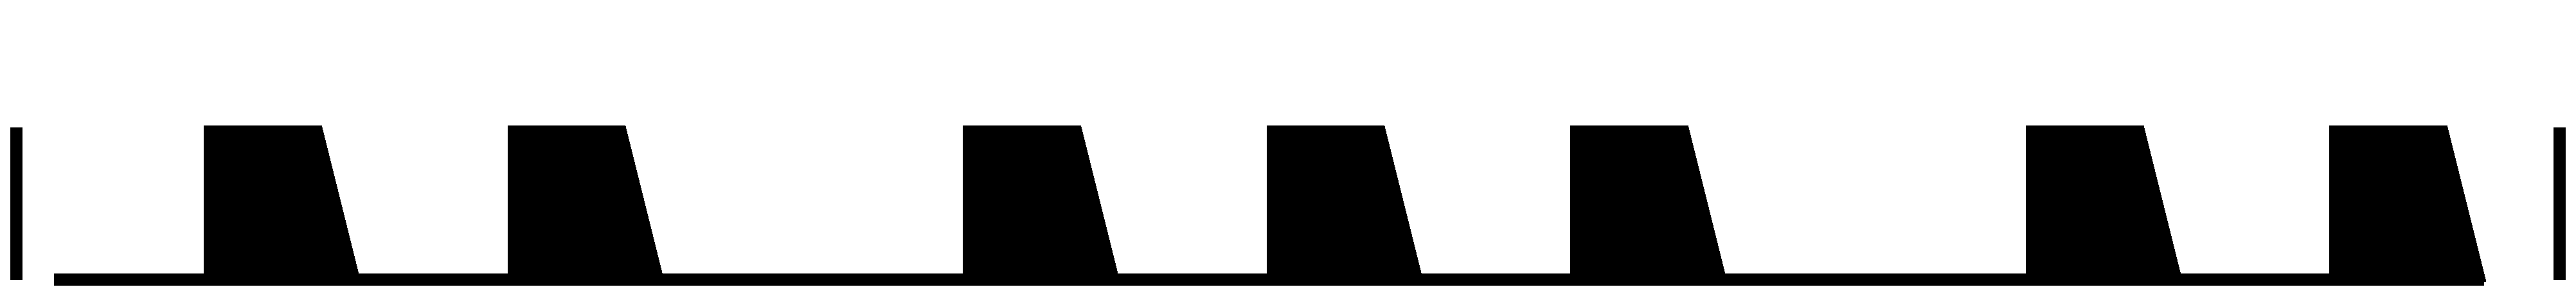
\includegraphics[width=\textwidth]{chapters/cap-musica-basica/forma-figurasexample2.eps}
        \caption{Sequencia rítmica usando um gráfico indicando a potencia do sonido.}
        \label{fig:forma-figurasexample2}
    \end{subfigure}
    \caption{Sequencia rítmica.}\label{fig:total-figurasexample2}
\end{figure}


Ate agora todos os exemplos foram sequencias rítmicas, 
pois não exploramos a possibilidade de variar a altura dos sons;
para poder explorar esta possibilidade devemos ter claro o conceito de pauta,
para que cada figura musical, 
além de nos proporcionar uma informação da \hyperref[sec:pos:Duracion]{\textbf{duração}}  dos sons, 
também nos de informação da \hyperref[sec:pos:Altura]{\textbf{altura}}  destes. 
Tendo estes dois fatores, altura e duração, podemos criar \hyperref[sec:pos:Melodia]{\textbf{melodias}}.

\begin{tcbinformation}
O mistério de como distinguir a pausa de mínima (\HaPa) e a pausa de semibreve (\GaPa),
será esclarecido quando desenhemos estes na \hyperref[sec:pauta]{\textbf{pauta}}, ver Seção \ref{sec:tipospauta}.
\end{tcbinformation}

\subsection{Ponto de aumento}
\index{Música!Ponto de aumento}
\label{subsec:pontoaumento}
O ponto de aumento é um simbolo que é colocado ao lado direito de uma figura musical ou pausa, 
e este indica um aumento do 50\% na duração \cite[pp. 25]{cardoso1973curso}.
A Tabela \ref{tab:notaspontoadas} mostra esta relação entre as durações.

\begin{table}[h]
\centering
\begin{tabular}{|c||c||c|}
\hline
Duração & Figura & Pausa \\ \hline
\hline
$\frac{3}{2}S$    & \Ganz. =  \Ganz + \Halb   & \GaPa. = \GaPa + \HaPa\\ \hline
$\frac{3}{4}S$    & \Halb. =  \Halb + \Vier   & \HaPa. = \HaPa + \ViPa  \\ \hline
$\frac{3}{8}S$    & \Vier. =  \Vier + \Acht   & \ViPa. = \ViPa + \AcPa  \\ \hline
$\frac{3}{16}S$   & \Acht. =  \Acht + \Sech   & \AcPa. = \AcPa + \SePa  \\ \hline
$\frac{3}{32}S$   & \Sech. =  \Sech + \Zwdr   & \SePa. = \SePa + \ZwPa  \\ \hline
\end{tabular}
\caption{Duração e símbolos de algumas figuras musicais com ponto de aumento}
\label{tab:notaspontoadas}
\end{table}

Da mesma forma que usamos um ponto de aumento, podem ser usados dois ou três pontos de aumento.
\begin{example}
Se usamos dois pontos de aumento a duração de uma nota cresce um 75\%, assim: \Halb.. = \Halb + \Vier + \Acht
\end{example}
\begin{example}
Se usamos tres pontos de aumento a duração de uma nota cresce um 87.5\%, assim: \Vier... = \Vier + \Acht + \Sech + \Zwdr
\end{example}
